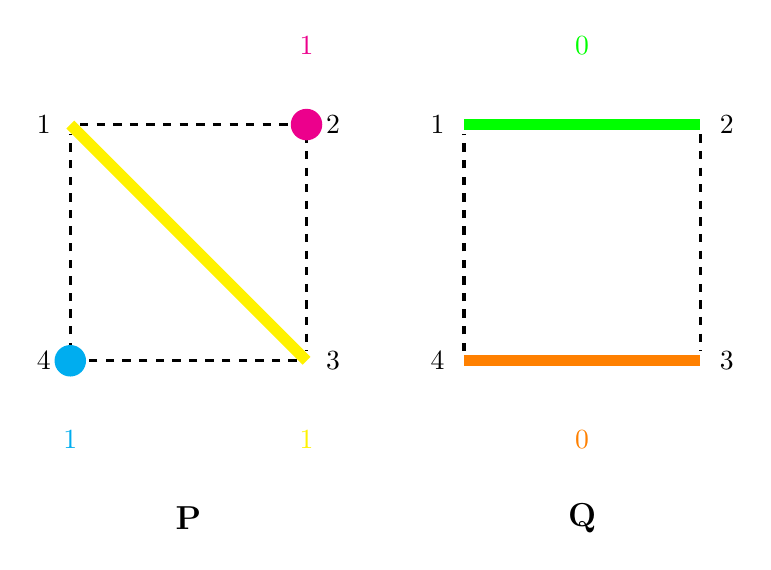
\begin{tikzpicture}[scale=1]
    \node at (1.5,-2) {\large $\mathbf{P}$};
    \node [label = left : {$1$}] (1)
        at (0,3) {};
    \node [label = right : {$2$}] (2)
        at (3,3) {};
    \node [label = right : {$3$}] (3)
        at (3,0) {};
    \node [label = left : {$4$}] (4)
        at (0,0) {};
    \draw [dashed][very thick] (1) -- (2) -- (3) -- (4)
        -- (1);
    \fill [color = cyan] (0,0) circle (0.2);
    \fill [color = magenta] (3,3) circle (0.2);
    \draw [color = yellow][line width = 4pt] (0,3) -- (3,0);
    \node [color = cyan] at (0, -1) {$1$};
    \node [color = magenta] at (3, 4) {$1$};
    \node [color = yellow] at (3, -1) {$1$};

    \node at (6.5,-2) {\large $\mathbf{Q}$};
    \node [label = left : {$1$}] (1b)
        at (5,3) {};
    \node [label = right : {$2$}] (2b)
        at (8,3) {};
    \node [label = right : {$3$}] (3b)
        at (8,0) {};
    \node [label = left : {$4$}] (4b)
        at (5,0) {};
    \draw [dashed][very thick] (1b) -- (2b) -- (3b) -- (4b)
        -- (1b);
    \draw [color = green][line width = 4pt] (5,3) -- (8,3);
    \draw [color = orange][line width = 4pt] (5,0) -- (8,0);
    \node [color = green] at (6.5, 4) {$0$};
    \node [color = orange] at (6.5, -1) {$0$};
  \end{tikzpicture}